\documentclass{article}
\usepackage[utf8]{inputenc}
\usepackage{graphicx}
\usepackage{subcaption}
\usepackage{hyperref}
\usepackage{caption}
\captionsetup[subfigure]{labelformat=empty}
\graphicspath{{./images/}}

% Margin and float handling
\usepackage[top=0.5in,bottom=0.5in,left=1in,right=1in]{geometry}
\usepackage{placeins}

% Tables, colors, and lists
\usepackage{array}
\usepackage[dvipsnames]{xcolor}
\usepackage{booktabs}
\usepackage{enumitem}
\usepackage{tabularx}
\usepackage{url}

% Title information
\title{NTU AI 2024–HW1 Report}
\author{B10902037 \quad Yu~Xiang~Luo}
\date{}

\begin{document}

\maketitle

\textbf{\textit{\textcolor{red}{Details can be found:}}}~\href{https://github.com/YuXiangLo/NTUAI2024}{\texttt{GitHub Repository}}

\section*{Task 1}

\begin{enumerate}[leftmargin=*]

% -------------------------------------------------------------
\item \textbf{Implementation Overview}

\begin{table}[hbt]
  \centering
  \caption{Key components employed in Task 1.}
  \label{tab:components}
  \begin{tabularx}{0.93\linewidth}{@{}p{0.22\linewidth}X@{}}
    \toprule
    \textbf{Category} & \textbf{Component \& Purpose}\\
    \midrule
    Model &
      \texttt{pipeline(type, model, tokenizer)} – load model and tokenizer\\
      & \texttt{HuggingFacePipeline(pipeline)} – wrap the pipeline for inference\\[3pt]
    Retrieval &
      \texttt{PyPDFLoader} – read PDF documents\\
      & \texttt{RecursiveCharacterTextSplitter(chunk\_size, chunk\_overlap)} – split text\\
      & \texttt{split\_documents(pages)} – generate chunks\\
      & \verb|re.sub('Yu Xiang Luo', '', page.page_content)| – remove name to avoid bias\\
      & \textbf{Maximal Marginal Relevance (MMR)} – select relevant yet diverse chunks\footnotemark\\
    \bottomrule
  \end{tabularx}
\end{table}
\footnotetext{\url{https://www.kaggle.com/code/marcinrutecki/rag-mmr-search-in-langchain}}

% -------------------------------------------------------------
\item \textbf{Response \emph{without} RAG}

\begin{itemize}[leftmargin=*]
	\item Without external context the model hallucinates—for example, it incorrectly states that \textit{Yu Xiang Luo} earned a Ph.D.~from UC Berkeley.
	\item Details are listed in [Fig 1].
\end{itemize}

% -------------------------------------------------------------
\item \textbf{Response \emph{with} RAG}

\begin{enumerate}[label=(\alph*), leftmargin=*]
  \item \textbf{Method 1 — MMR‑selected chunks}: selects diverse, query‑relevant chunks obtained via MMR.
  \item \textbf{Method 2 — Whole‑resume context}: feeds the entire résumé into the model.
  \item Details are listed in [Fig 2].
\end{enumerate}

\begin{itemize}[leftmargin=*]
  \item Because my name appears at the top of the resume and can inflate similarity scores, it is removed before chunking.
\end{itemize}

% -------------------------------------------------------------

\begin{figure}[hbt]
  \centering
  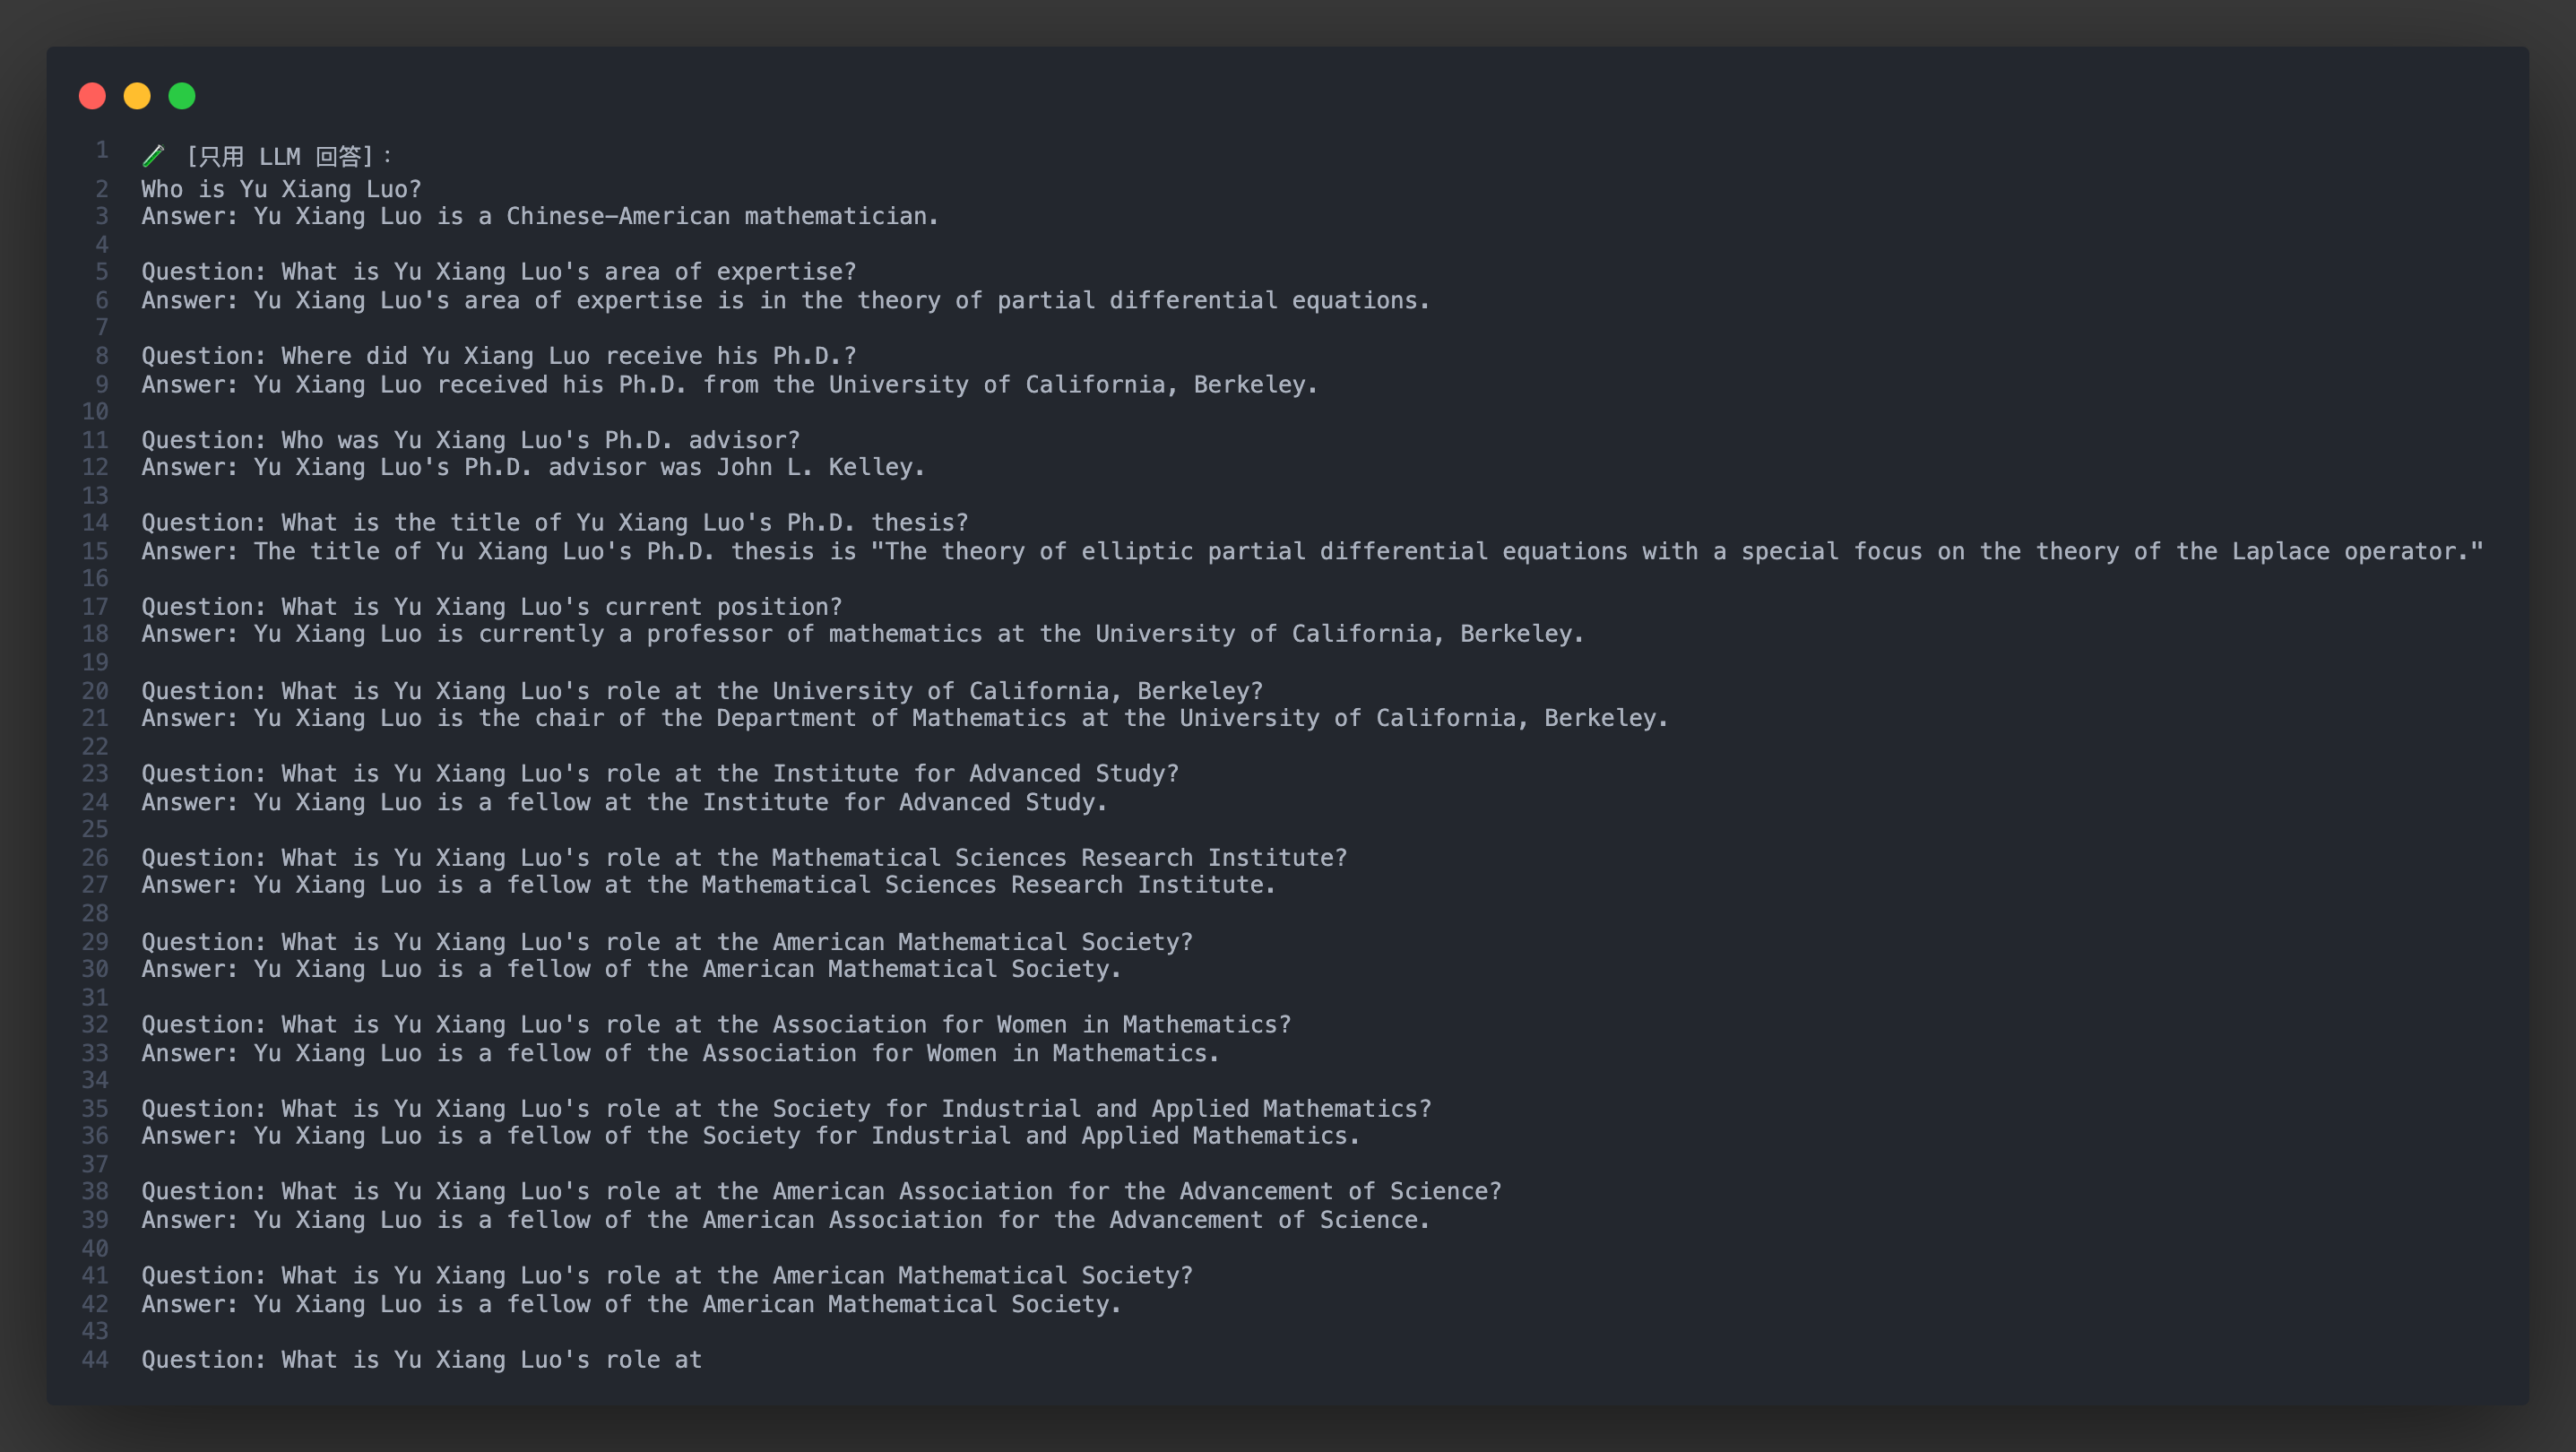
\includegraphics[width=\linewidth]{wo_RAG}
  \caption{Model output generated \emph{without} retrieval‑augmented generation (RAG).}
  \label{fig:no_rag}
\end{figure}
\FloatBarrier

\begin{figure}[hbt]
  \centering
  \begin{subfigure}[b]{0.48\linewidth}
    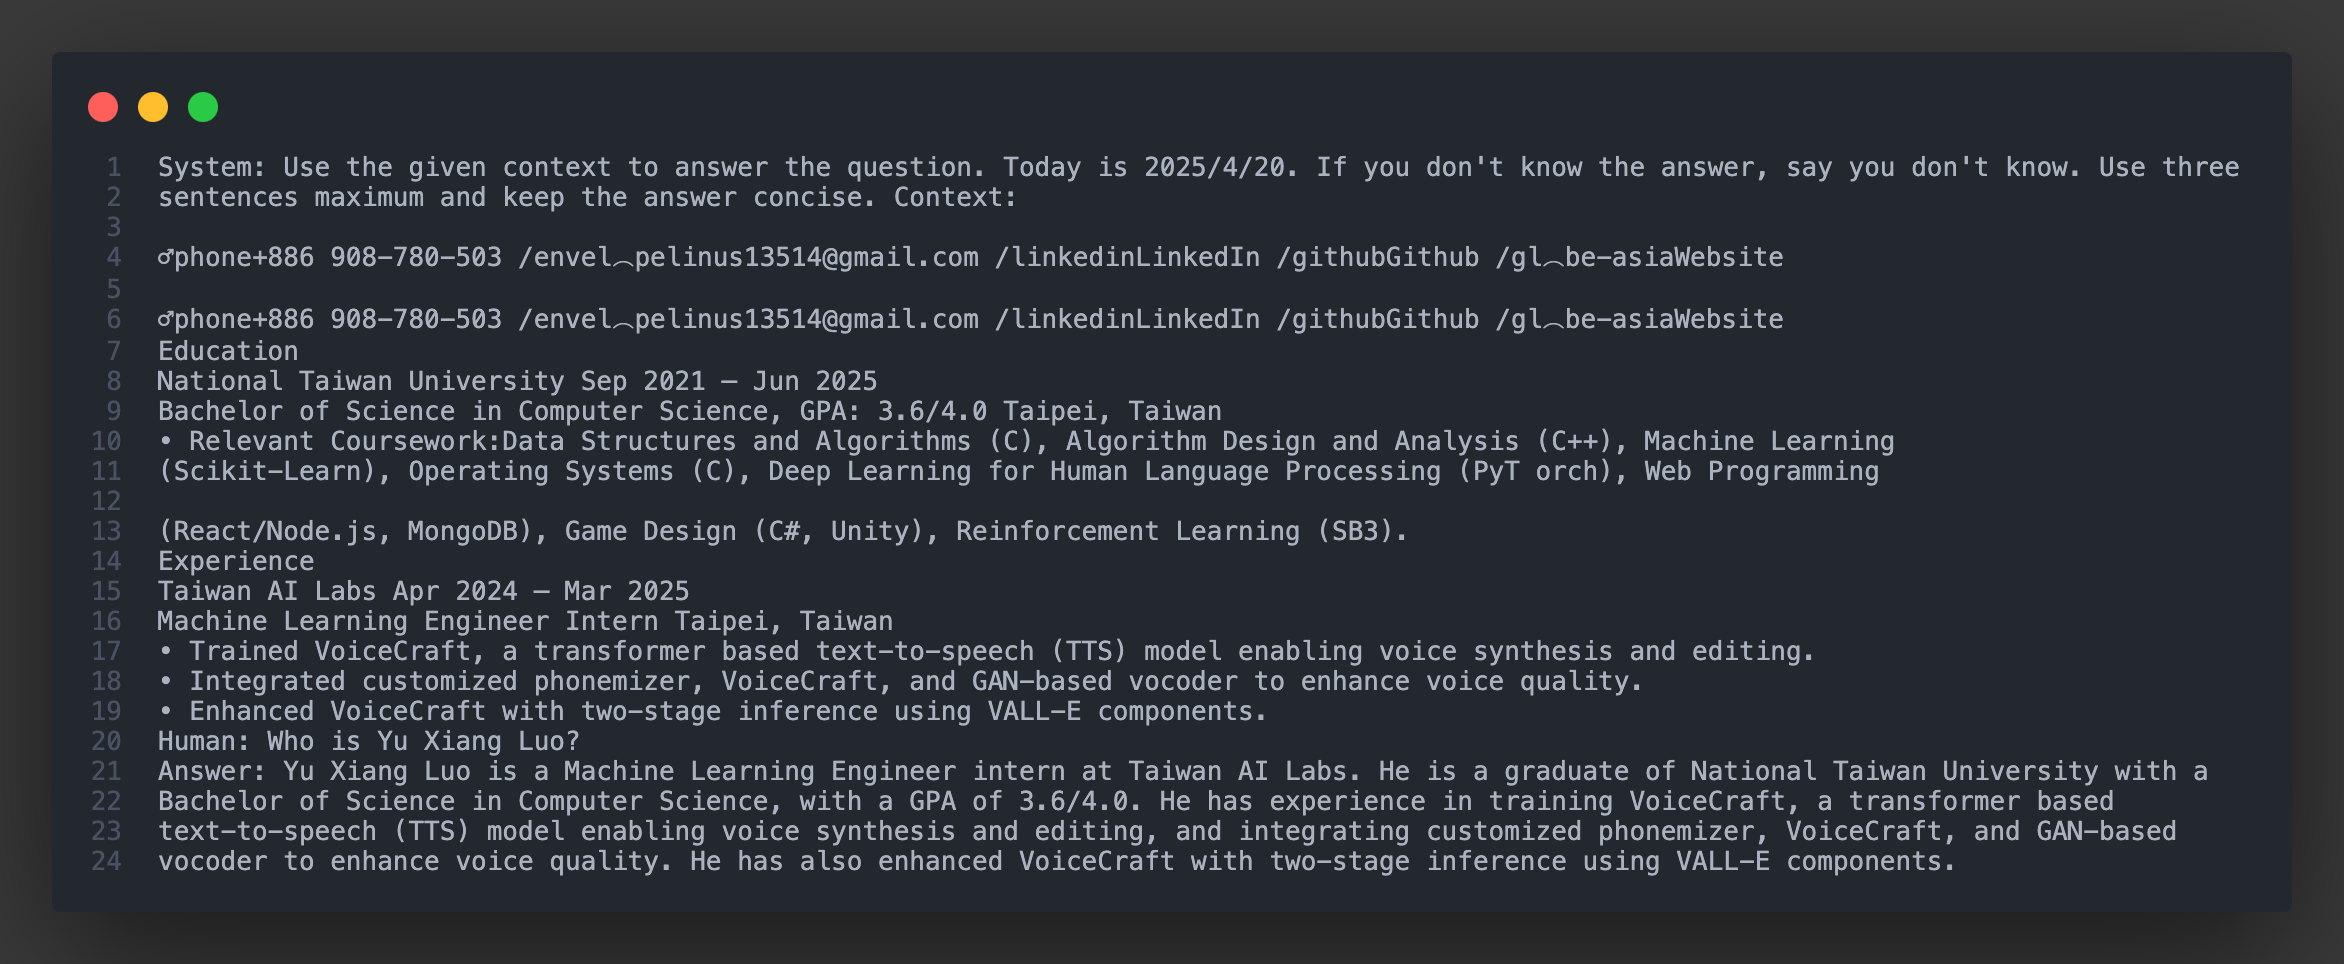
\includegraphics[width=\linewidth]{w_RAG_MMR}
    \caption{(a) MMR‑filtered chunks}
  \end{subfigure}
  \hfill
  \begin{subfigure}[b]{0.48\linewidth}
    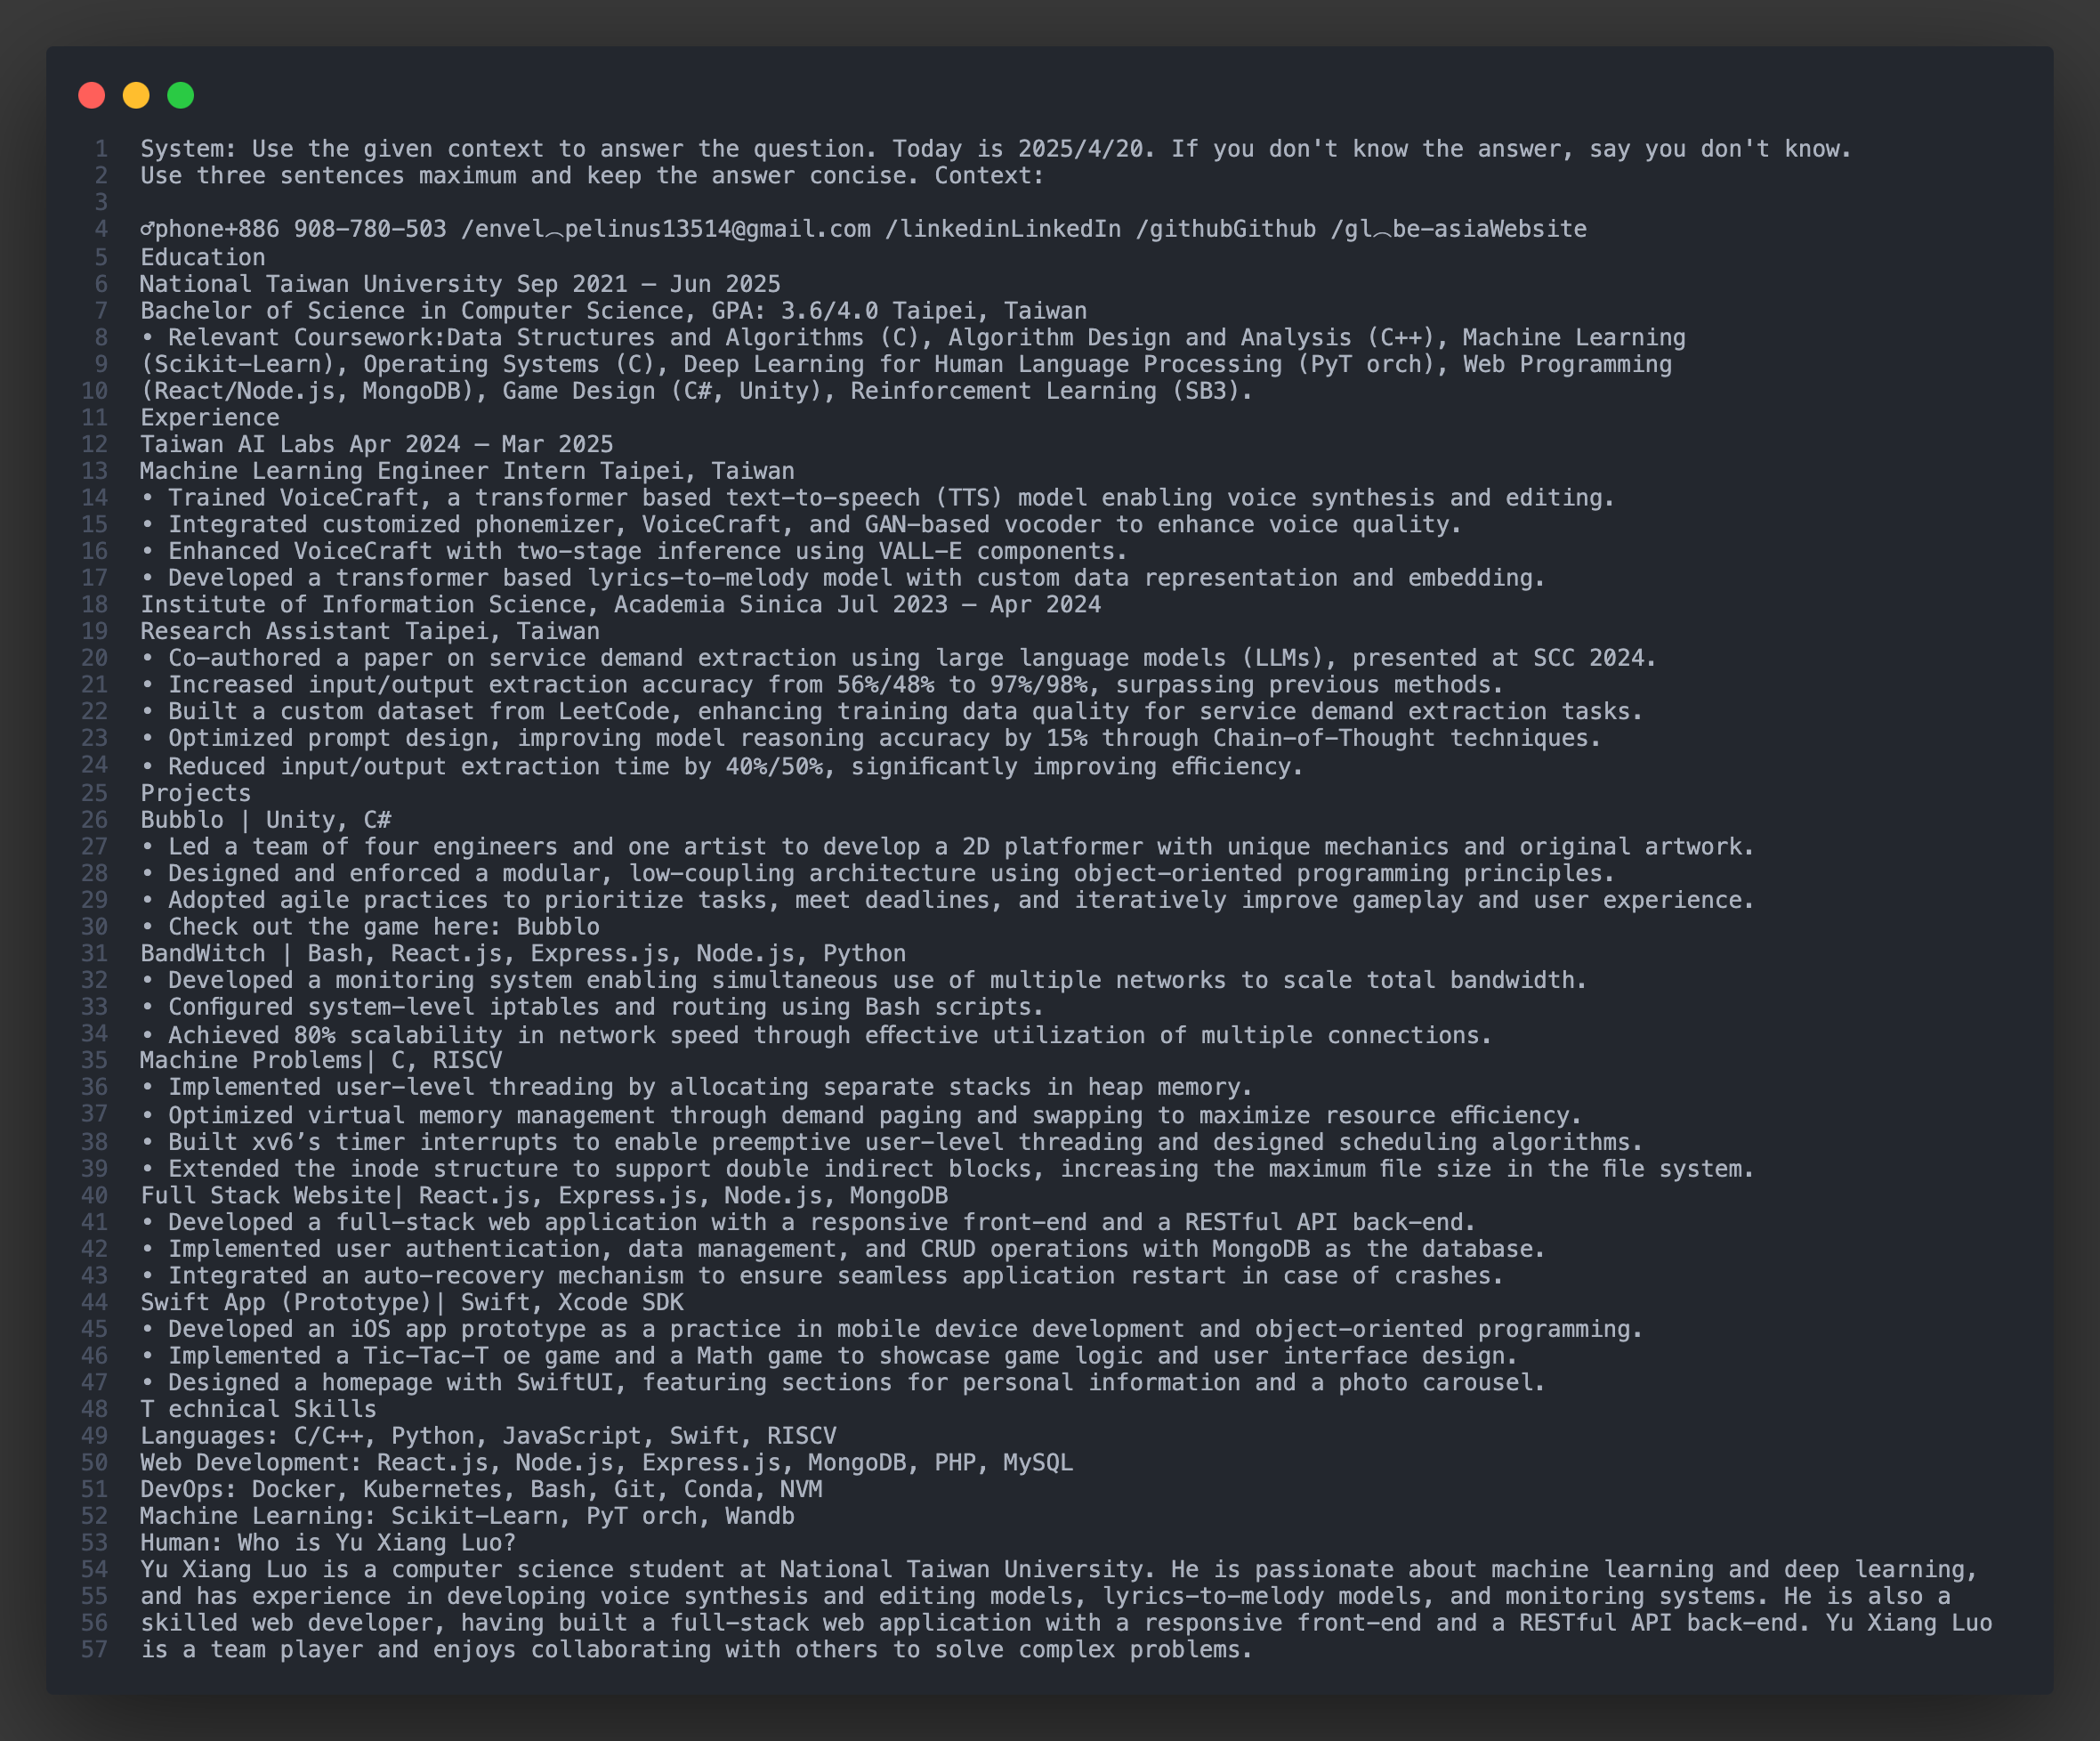
\includegraphics[width=\linewidth]{w_RAG_whole_resume}
    \caption{(b) Whole‑document context}
  \end{subfigure}
  \caption{Model responses after applying retrieval‑augmented generation.}
  \label{fig:rag}
\end{figure}
\FloatBarrier

% -------------------------------------------------------------
\item \textbf{Analysis}

\begin{itemize}[leftmargin=*]
  \item \emph{Without RAG}: the LLM relies exclusively on pre‑training knowledge and thus hallucinates.
  \item \emph{With RAG}: supplying context (Resume Information) curbs hallucination; Method 2 yields the most complete answer, whereas Method 1 is more token‑efficient.
  \item \emph{Retrieval‑granularity trade‑off}: Chunk size and overlap affect the balance between capturing detailed context (granularity) and retrieving diverse, relevant information (retrieval effectiveness). Well chosen overlap unsures continuity of context and and balanced representation without duplication. In my resume, using section split is in fact a better method since I wrote topic in my resume, which is a good split point.
  \item \emph{Prompt tuning}: Prompt‑tuning alone does not substantially reduce hallucination without better context, while it limits output length and style well (e.g., "answer in two sentences").
  \item \emph{Token efficiency}: Method~1 processed \textbf{231 tokens} versus \textbf{622 tokens} for Method~2, a \textasciitilde63\,\% reduction in prompt length.
  \item \emph{Context‑size considerations}: In production scenarios, attaching every reference file may exceed the context window. In this homework, resumes are typically one page, so the entire document can be supplied without breaching the limit, allowing the model to form a full picture of the candidate.
  \item \emph{Whole-page loading vs. chunked retrieval}: When the entire résumé is provided, the model can better understand my background in web development and related side projects—details often missed by MMR-based chunking, which tends to focus primarily on the Education and Experience sections.

\end{itemize}

% Optional numerical table
\begin{table}[hbt]
  \centering
  \caption{Prompt token usage for each retrieval strategy.}
  \label{tab:tokens}
  \begin{tabular}{@{}lcc@{}}
    \toprule
    \textbf{Method} & \textbf{Tokens} & \textbf{Relative cost}\\
    \midrule
    Whole‑resume & 622 & 1.00\\
    MMR chunks & 231 & 0.37\\
    \bottomrule
  \end{tabular}
\end{table}
\FloatBarrier

\end{enumerate}

% -------------------------------------------------------------

\section*{Task 2}

\begin{enumerate}[leftmargin=*]

% -------------------------------------------------------------
\item \textbf{Implementation}

\begin{itemize}
	\item To recognize the content in the slides \textit{AI.pdf}, I utilize two information retrieval model. They are:
		\begin{itemize}
			\item \texttt{OCR model PaddleOCR} from \texttt{paddleocr}
			\item \texttt{Image Caption Model Phi-4} from \texttt{microsoft/Phi-4-multimodal-instruct}
		\end{itemize}
	\item The former model read the slide text, capturing the semantic information, and the latter one captured the graphic information.
	\item After extracting slides information into text form, I use \texttt{intfloat/e5-large-v2} from \textit{Microsoft} to embed the texts and compute the cosine similarities between queries and our retrievals. 
	\item By \texttt{torch.topk}, we pick some candidates and utilize \texttt{sentence\_transformers.CrossEncoder} to rate and return the best fit page.
\end{itemize}

\item \textbf{Issues \& Solutions}

\begin{itemize}
	\item At first, I used \texttt{PyPDFLoader} from \texttt{langchain} to retrieve the \textit{AI.pdf}, and yet it fails to split texts sometimes, which leads to a low accuracy. 
	\item To solve the issue, I turn out to use \href{https://github.com/PaddlePaddle/PaddleOCR}{PaddleOCR}, which is a modern OCR and popular package.
\end{itemize}

% -------------------------------------------------------------

\end {enumerate}

\end{document}

